\chapter{Miniprojekt Del 3}

Vi har valgt en 1o sekunder lang lyd sekvens fra sangen "Uptown", som vores indgangssignal. 
Det er dette signal, der skal igennem equalizeren. 

\section{Design af filterne}
Til at designe de fem forskellige filter, bestemmes først knækfrekvenserne. Frekvensspektrumet skulle holdes inden for det hørebarespektrum, så dette spektrum dividerede vi med fem. Derefter kunne vi definere de forskellige knækfrekvenser til de forskellige filter. 
\\ \\
Da filterne ikke knækker skrapt ved knækfrekvensen, har vi valgt at de forskellige knækfrekvenser skal overlappe hinanden en lille smule (Figur 2.1), så vi får en lige linje, når vi plotter alle filterne ved siden af hinanden (Figur 2.3). 

\begin{figure}[H]
	\centering
	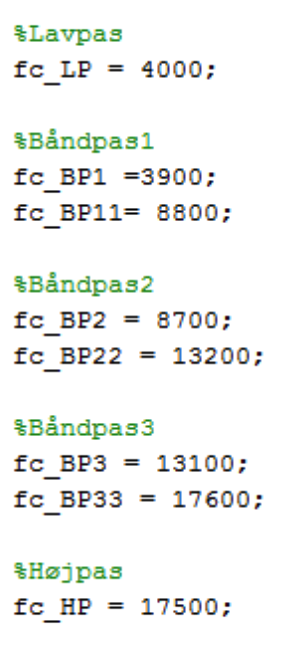
\includegraphics[width=0.2\textwidth]{Figur/Snip20151111_61}
	\caption{De valgte knækfrekvenser for de forskellige filter}
\end{figure}

Efter at have valgt knækfrekvenserne kunne filterne designes. Lavpasfilteret er designet som et IIR filter, mens de andre båndpas- og højpasfilter er designet som FIR filtere. Ved IIR filteret er der valgt en orden på 6 (N2). Ved FIR filterne er der valgt en orden på 1000 (N1). På Figur 2.2 kan koden for designet ses.  

\begin{figure}[H]
	\centering
	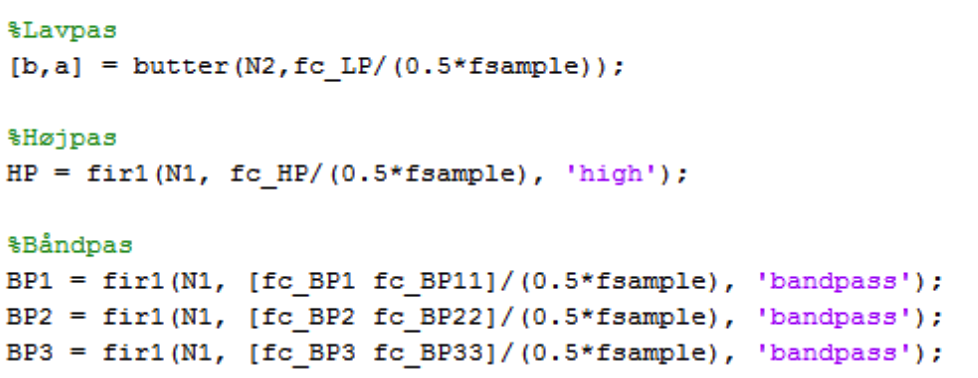
\includegraphics[width=0.8\textwidth]{Figur/Snip20151111_64}
	\caption{Designet af de fem filter}
\end{figure}

Hvis alle disse filter plottes i samme koordinatsystem, skulle der gerne komme en lige linje - altså at de hverken overlapper hinanden for meget eller for lidt (Figur 2.3). 

\begin{figure}[H]
	\centering
	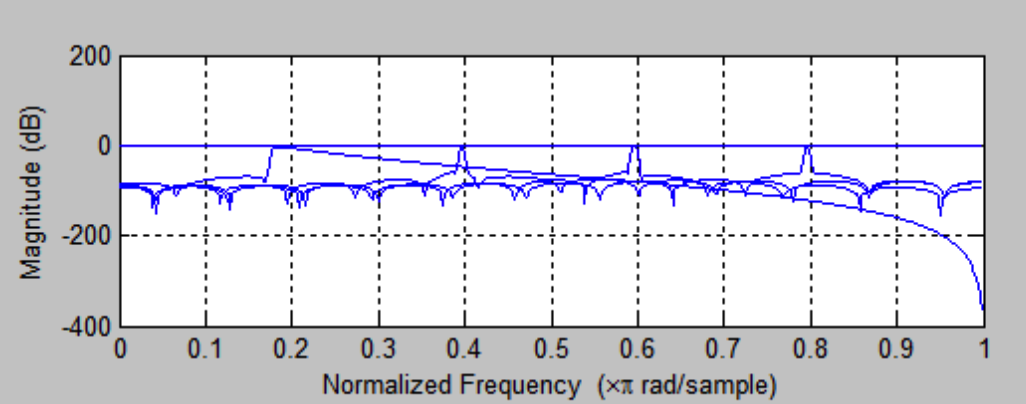
\includegraphics[width=0.8\textwidth]{Figur/Snip20151111_65}
	\caption{De fem filter plottet ved siden af hinanden}
\end{figure}


\section{Filtering af signalet}
Signalet skal nu igennem de fem forskellige filter, hvor så det samlede output er det, vi er interesseret i. 

\begin{figure}[H]
	\centering
	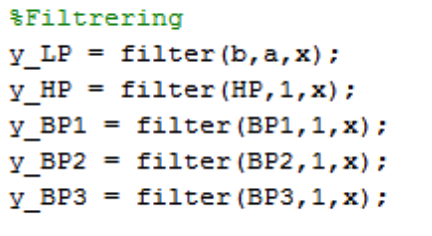
\includegraphics[width=0.6\textwidth]{Figur/Snip20151111_66}
	\caption{Signalet filteres gennem de fem filter}
\end{figure}

\begin{figure}[H]
	\centering
	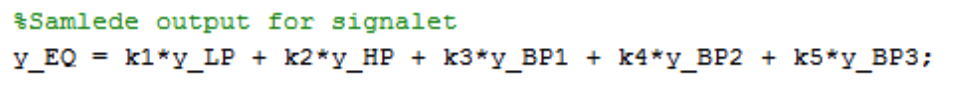
\includegraphics[width=0.8\textwidth]{Figur/Snip20151111_67}
	\caption{Det samlede filtreret signal}
\end{figure}

Det ufiltreret signal skal gerne være det sammen som det filtreret signalet, hvis alle forstærkningskoeficienterne er lig 1 (Figur 2.6 og 2.7).  

\begin{figure}[H]
	\centering
	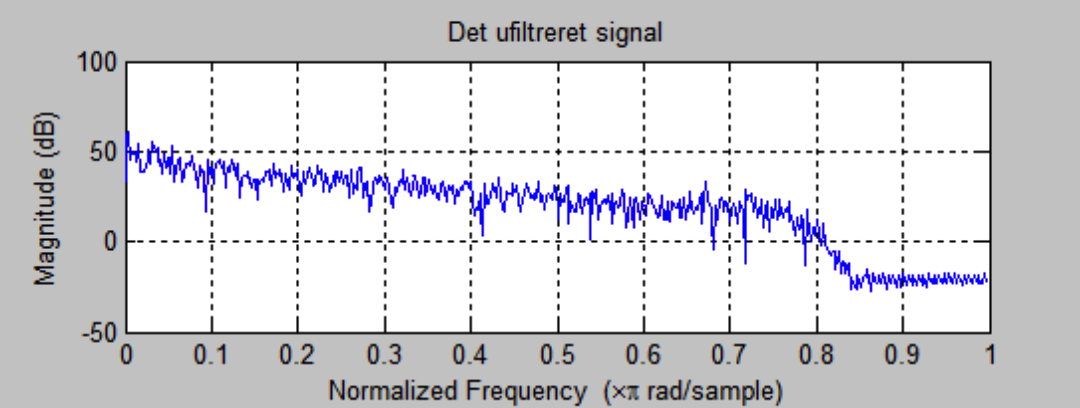
\includegraphics[width=0.8\textwidth]{Figur/Snip20151111_68}
	\caption{Det ufiltreret signal}
\end{figure}

\begin{figure}[H]
	\centering
	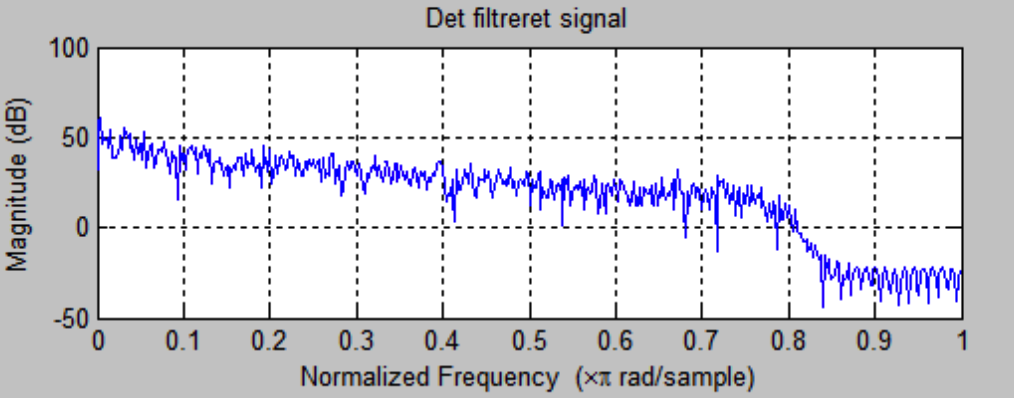
\includegraphics[width=0.8\textwidth]{Figur/Snip20151111_69}
	\caption{Det filtreret signal}
\end{figure}

Det er det samme bortset fra efter 0.8, men vores signal løber kun derhen til, så derfor kan vi godt antage, at de to er de samme. 
\\ \\
Hvis der så ændres på nogle af forstærkningskoeficienterne, vil vi se højere amplituder i det frekvensbånd, vi forstærker signalet. 
Fx ønskes der en forstærkning på 15 gange af de dybe toner (Bas) og af de høje toner, vil K1 og K2 ændres fra 1 til 10 og der vil forekomme større amplituder ved de lave frekvenser og de høje frekvenser (Figur 2.8). 

\begin{figure}[H]
	\centering
	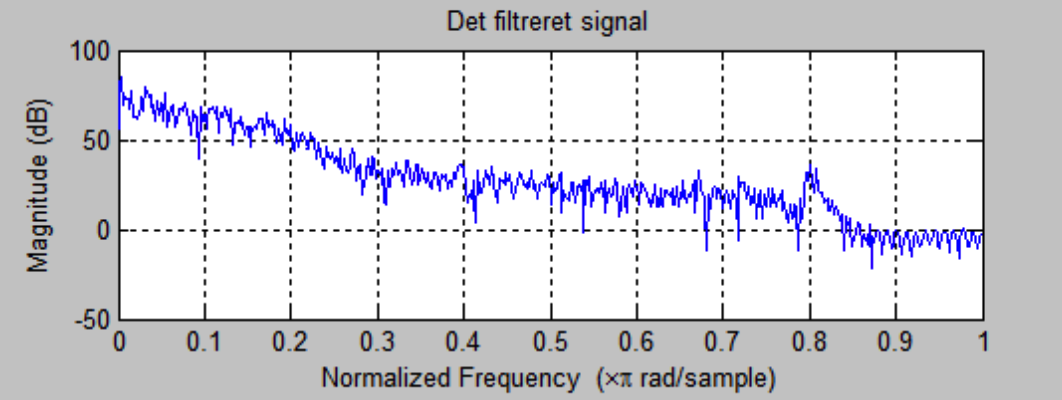
\includegraphics[width=0.8\textwidth]{Figur/Snip20151111_70}
	\caption{Det filtreret signal, hvor de dybe og høje toner er blevet forstærket med 15}
\end{figure}

Så man skal forestille sig, at forstærkningskoeficienterne er knapperne på et stereoanlæg, som man kan dreje på for at skrue op eller ned for de forskellige frekvenser (toner). 

\section{FFT af filtrene}
En af opgaverne i projektet var at vise amplitude og fase i frekvensdomænet for de forskellige filteret og samlede signal. Dette gøres ved at tage FFT af signalet og kører det igennem filtrene, der også har været igennem en FFT. 
Det inverse af det samlede signal af dette skulle gerne være det samme som det ufiltreret signal og det filtreret signal, hvor der ingen forstærkning var.  

\subsection{Lavpas filtreret}
For lavpas filtreret laves FFT'en lidt anderledes end ved de andre filtre, da det er et IIR filter. 

\begin{figure}[H]
	\centering
	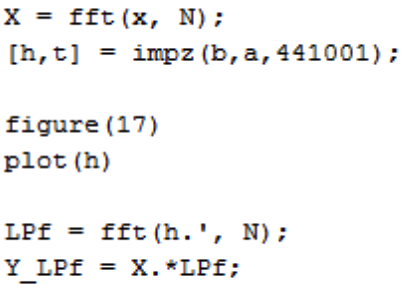
\includegraphics[width=0.6\textwidth]{Figur/Snip20151111_71}
	\caption{FFT af lavpas}
\end{figure}

Den første linje er, hvor der tages en FFT af selve signalet. Det er denne X, der benyttes i de andre filtre også. 
\\
I anden linje findes impulsresponsen for IIR filtreret, da det er denne man kan tage en FFT af. De 441001 er for at få sammen længde som selve signalet. 

\begin{figure}[H]
	\centering
	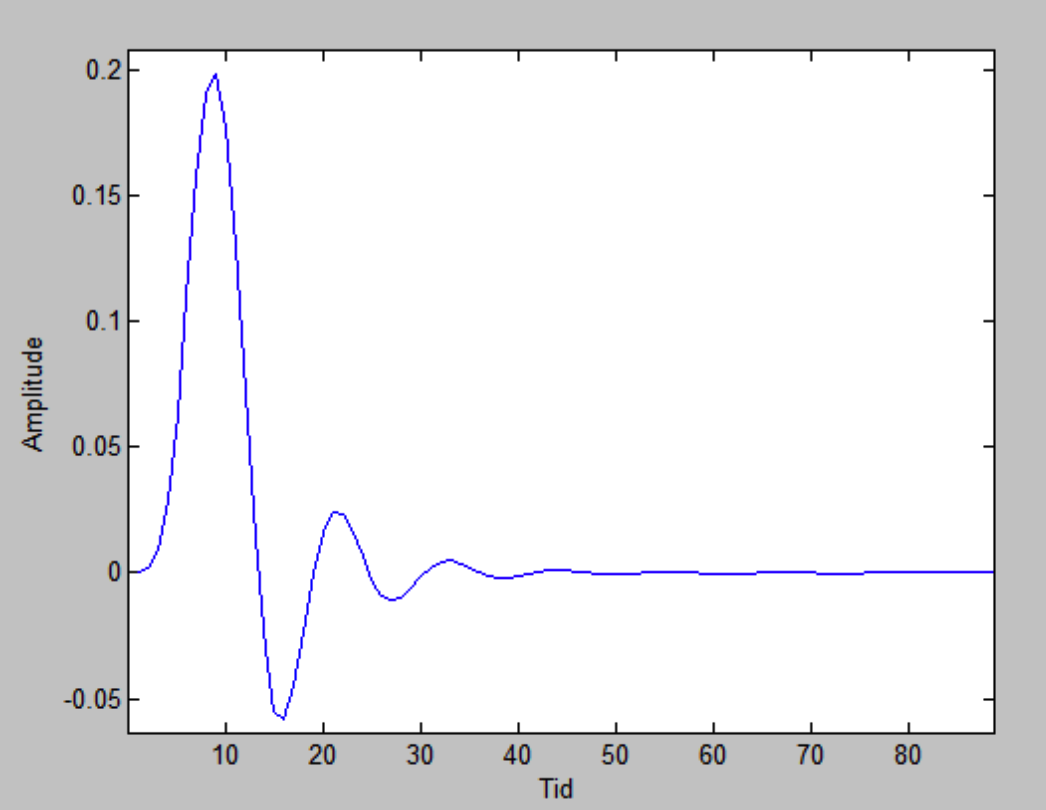
\includegraphics[width=0.8\textwidth]{Figur/Snip20151111_73}
	\caption{IIR lavpas filtrers impulsrespons}
\end{figure}

Efter at have fundet impulsresponsen kan man lave FFT'en. Det er femte linje, der står for det i Figur 2.9. 
I sjette linje ganger man signalet sammen med filteret, der begge har været igennem FFT, så man får outputsignalet. 

\begin{figure}[H]
	\centering
	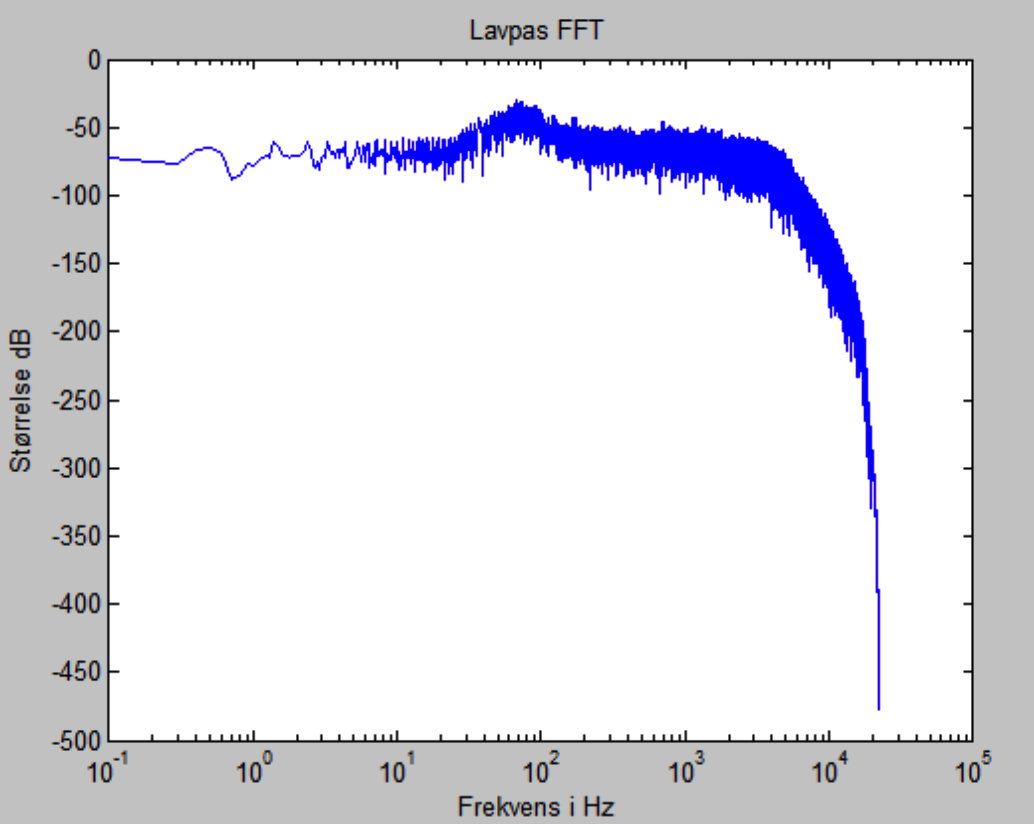
\includegraphics[width=0.8\textwidth]{Figur/Snip20151111_74}
	\caption{Amplituden for Lavpas FFT}
\end{figure}

Her kan man se, at det er er lave frekvenser, der bliver lukket igennem. 

\begin{figure}[H]
	\centering
	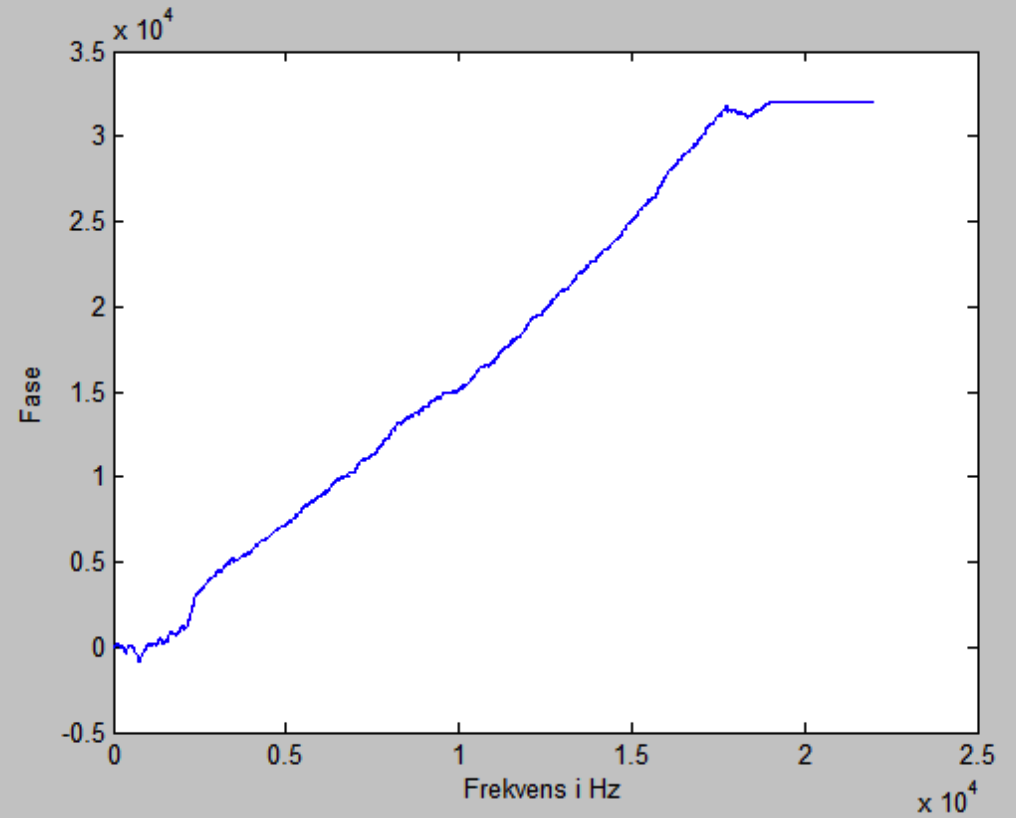
\includegraphics[width=0.8\textwidth]{Figur/Snip20151111_75}
	\caption{Fasen for Lavpas FFT}
\end{figure}

\subsection{Båndpasfiltre 1}
For resten af filterne tager man FFT, som normalt og ganger X og FFT af filterne sammen. 

\begin{figure}[H]
	\centering
	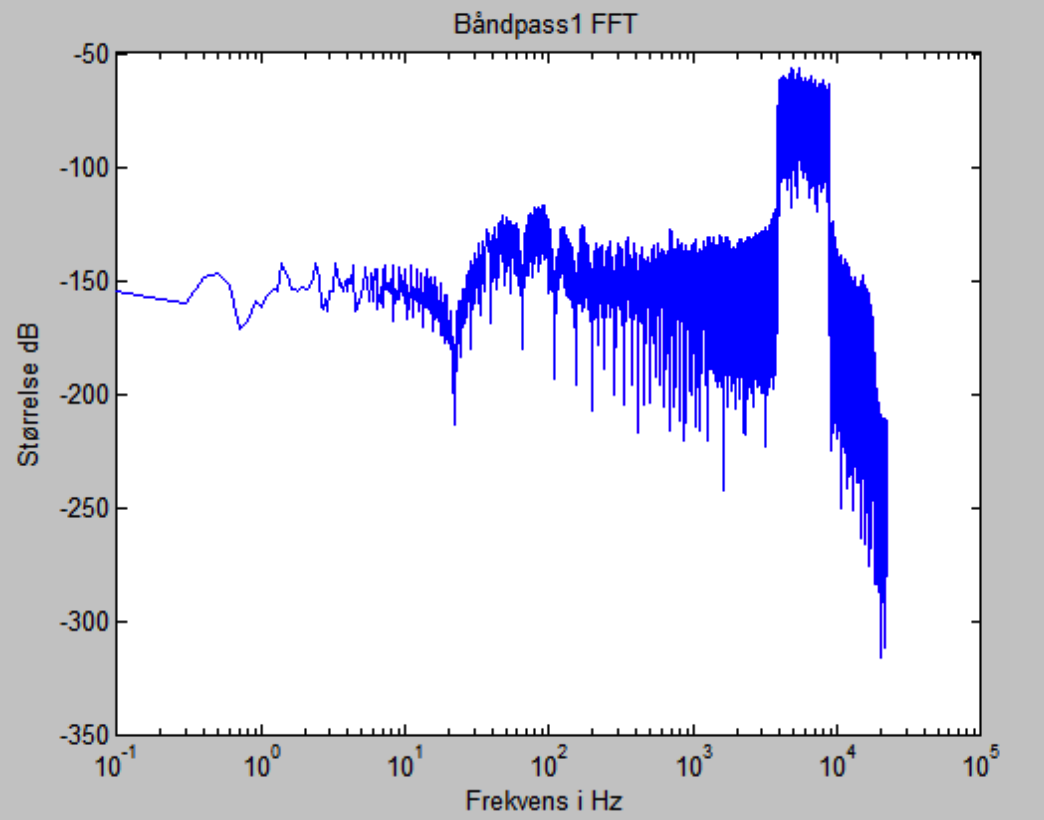
\includegraphics[width=0.8\textwidth]{Figur/Snip20151111_76}
	\caption{Amplituden for Båndpas1 FFT}
\end{figure}

Her er frekvensintervallet fra 3800 til 9000 forstærket mere end resten af signalet. 

\begin{figure}[H]
	\centering
	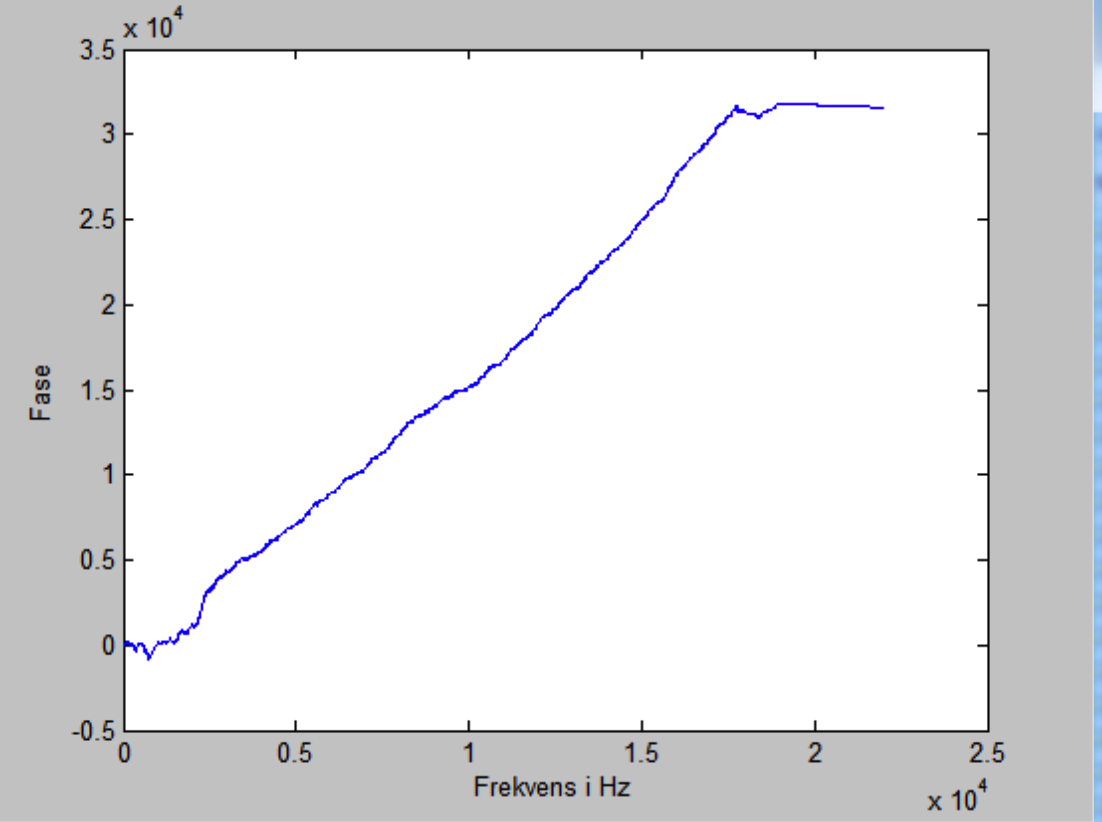
\includegraphics[width=0.8\textwidth]{Figur/Snip20151111_77}
	\caption{Fasen for Båndpas1 FFT}
\end{figure}

\subsection{Båndpasfiltre 2}

\begin{figure}[H]
	\centering
	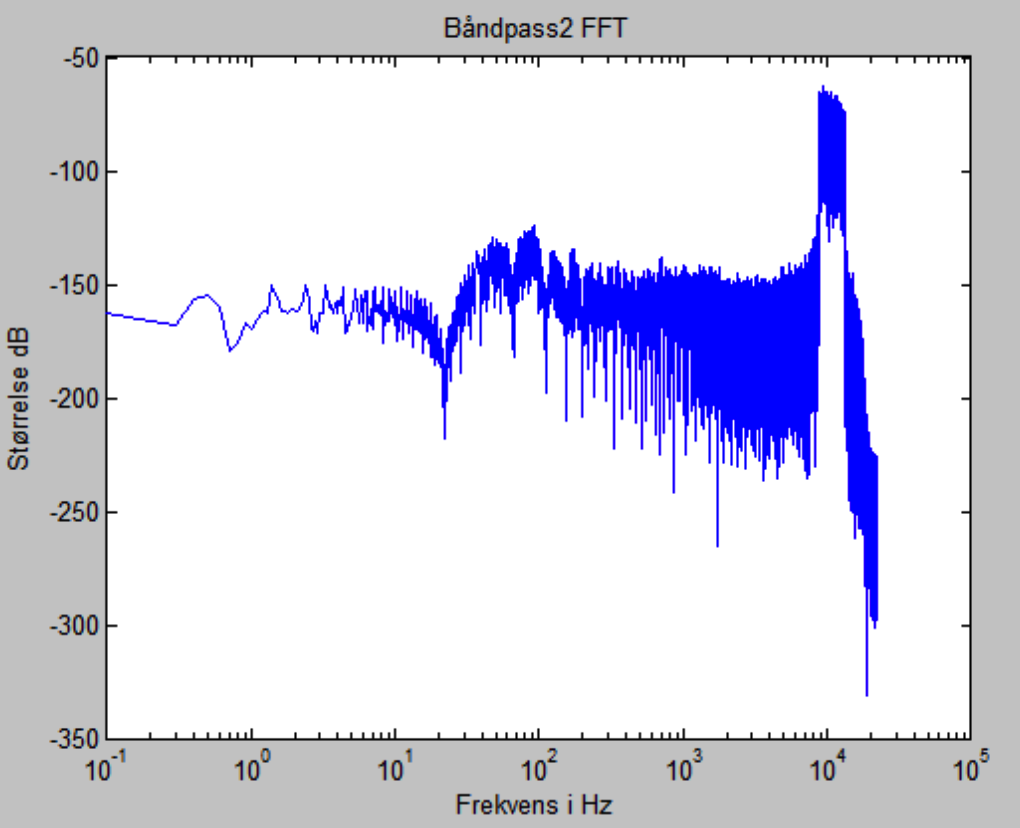
\includegraphics[width=0.8\textwidth]{Figur/Snip20151111_78}
	\caption{Amplitude for Båndpas2 FFT}
\end{figure}

Her er frekvensintervallet fra 8600 til 13000 forstærket mere end resten af signalet. 

\begin{figure}[H]
	\centering
	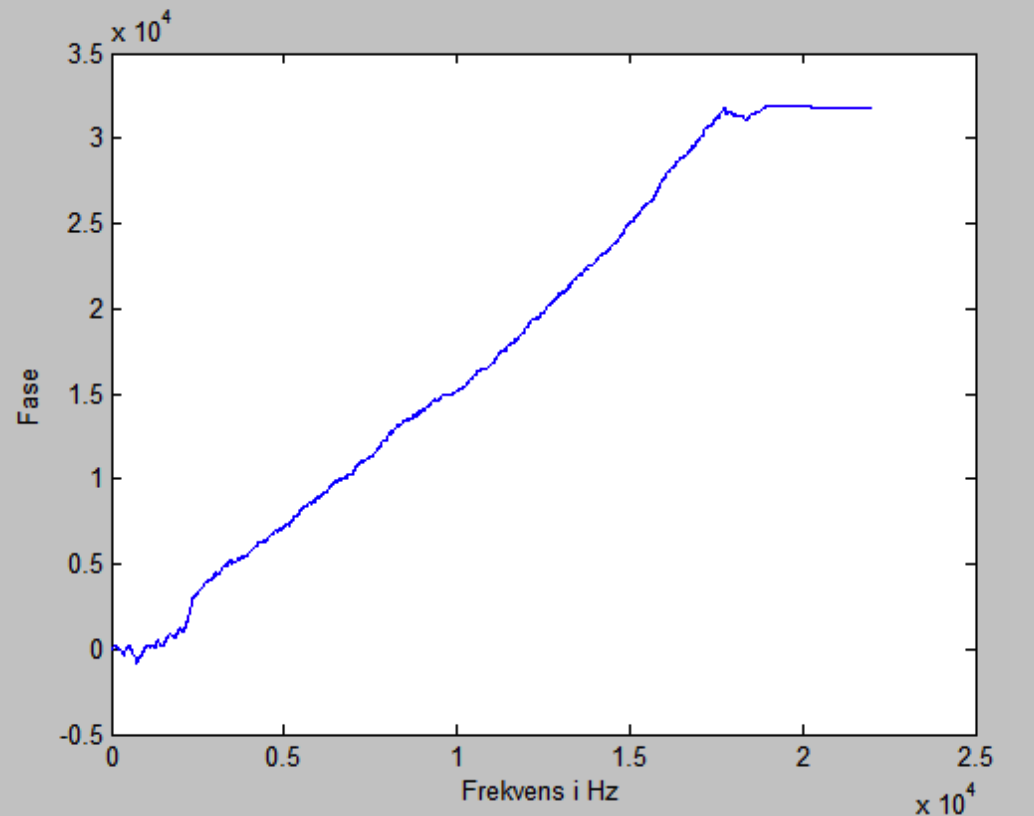
\includegraphics[width=0.8\textwidth]{Figur/Snip20151111_79}
	\caption{Fasen for Båndpas2 FFT}
\end{figure}

\subsection{Båndpasfiltre 3}

\begin{figure}[H]
	\centering
	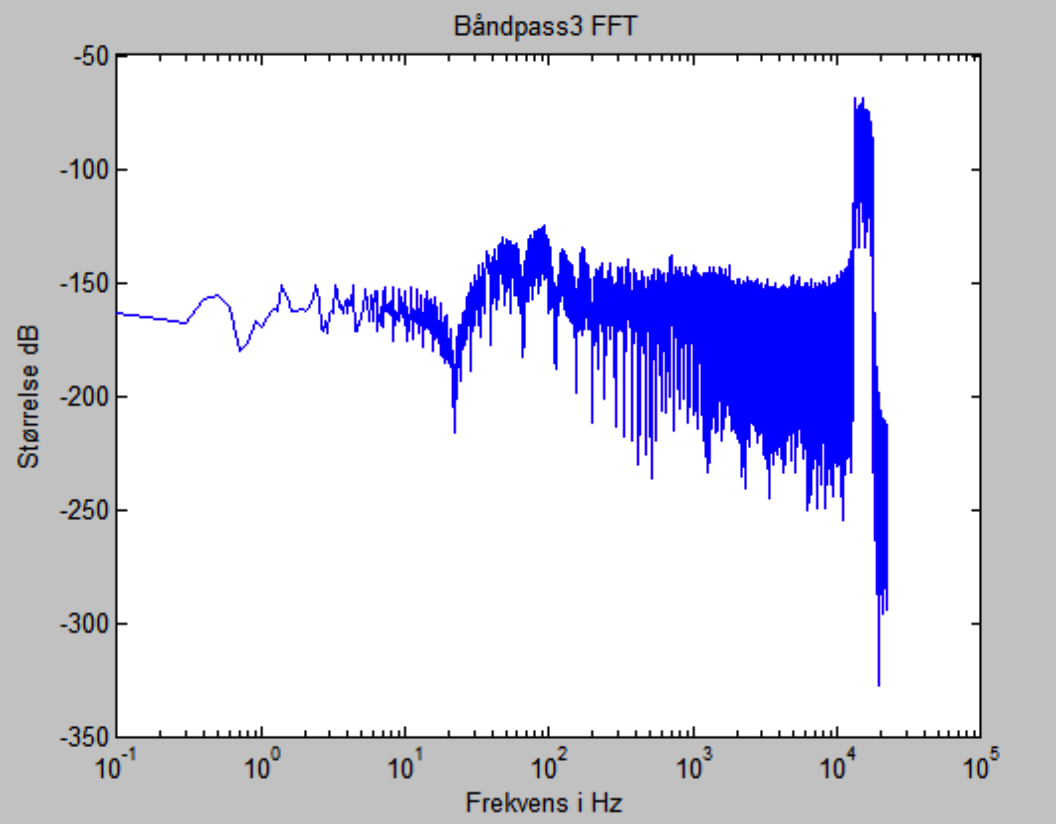
\includegraphics[width=0.8\textwidth]{Figur/Snip20151111_80}
	\caption{Amplituden for Båndpas3 FFT}
\end{figure}

Her er frekvensintervallet fra 13000 til 17000 forstærket mere end resten af signalet. 

\begin{figure}[H]
	\centering
	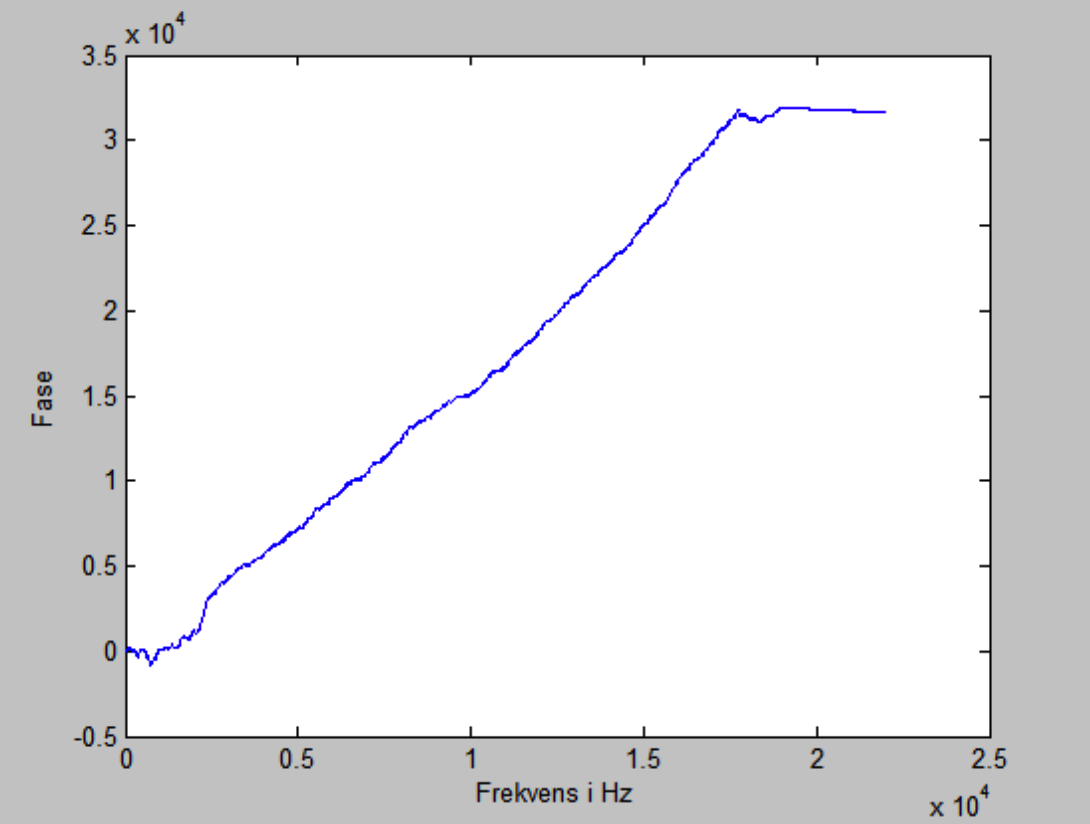
\includegraphics[width=0.8\textwidth]{Figur/Snip20151111_81}
	\caption{Fasen for Båndpas3 FFT}
\end{figure}

\subsection{Højpasfiltret}

\begin{figure}[H]
	\centering
	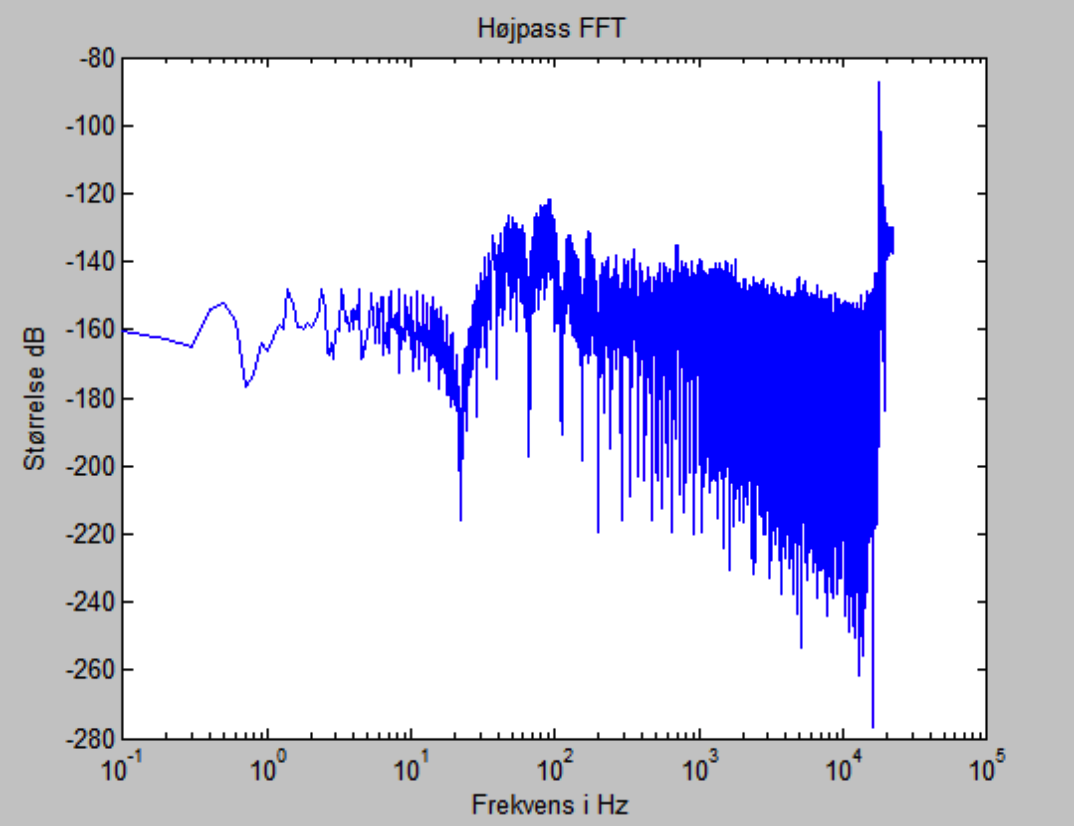
\includegraphics[width=0.8\textwidth]{Figur/Snip20151111_82}
	\caption{Amplituden for Højpas FFT}
\end{figure}

Her er det frekvenserne fra 17000 og op efter i signalet, der er blevet forstærket. 

\begin{figure}[H]
	\centering
	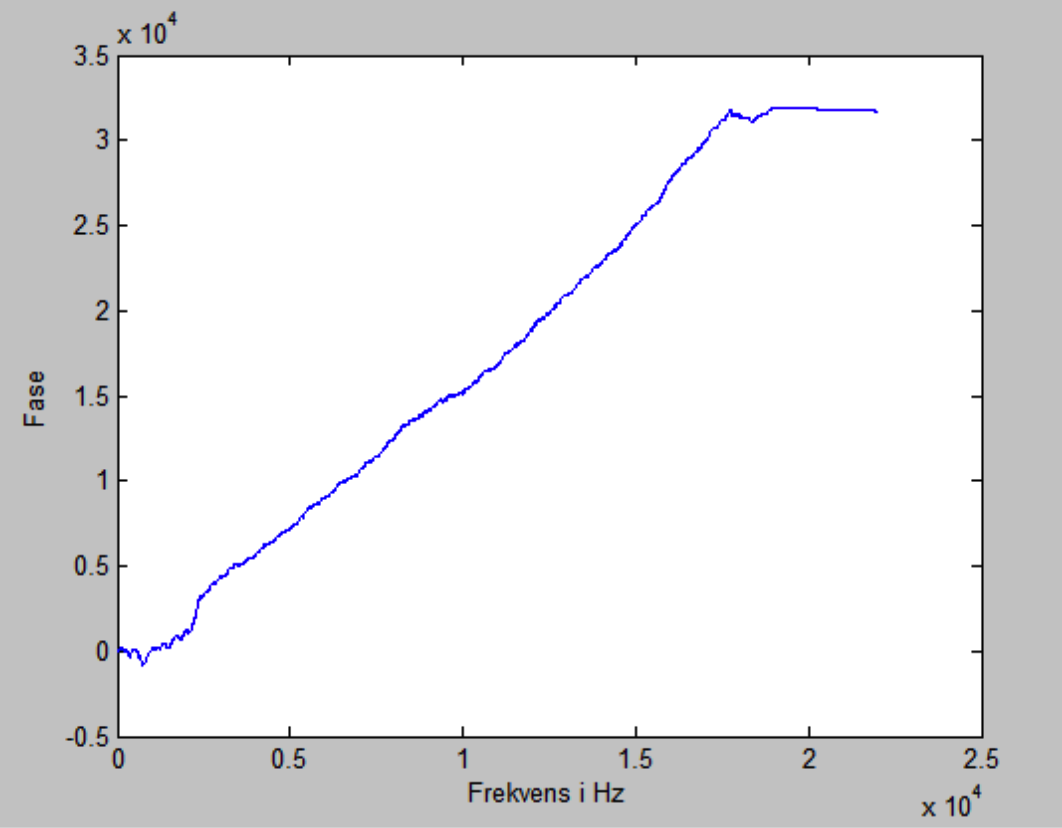
\includegraphics[width=0.8\textwidth]{Figur/Snip20151111_83}
	\caption{Fasen for højpas FFT}
\end{figure}

\section{Det samlede signal}
For at finde det samlede output for signalet efter FFT gøres ligesom før (Figur 2.21)

\begin{figure}[H]
	\centering
	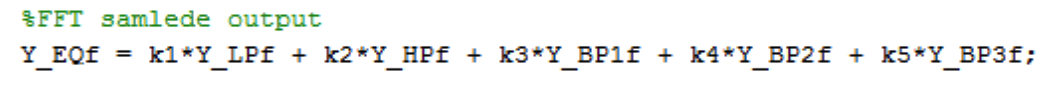
\includegraphics[width=0.8\textwidth]{Figur/Snip20151111_86}
	\caption{Ligning for det samlede signal}
\end{figure}

Dette plottes og kan ses på Figur 2.22 og 2.23. 

\begin{figure}[H]
	\centering
	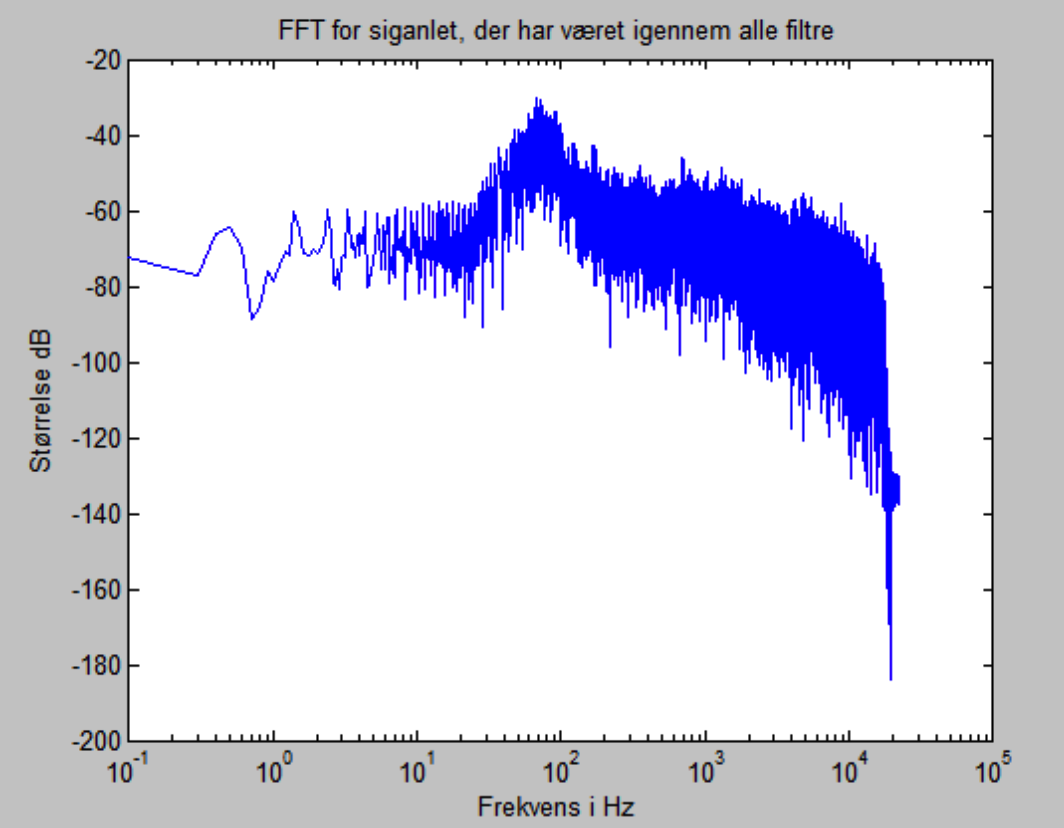
\includegraphics[width=0.8\textwidth]{Figur/Snip20151111_84}
	\caption{Amplituden for det samlede signal, FFT}
\end{figure}

\begin{figure}[H]
	\centering
	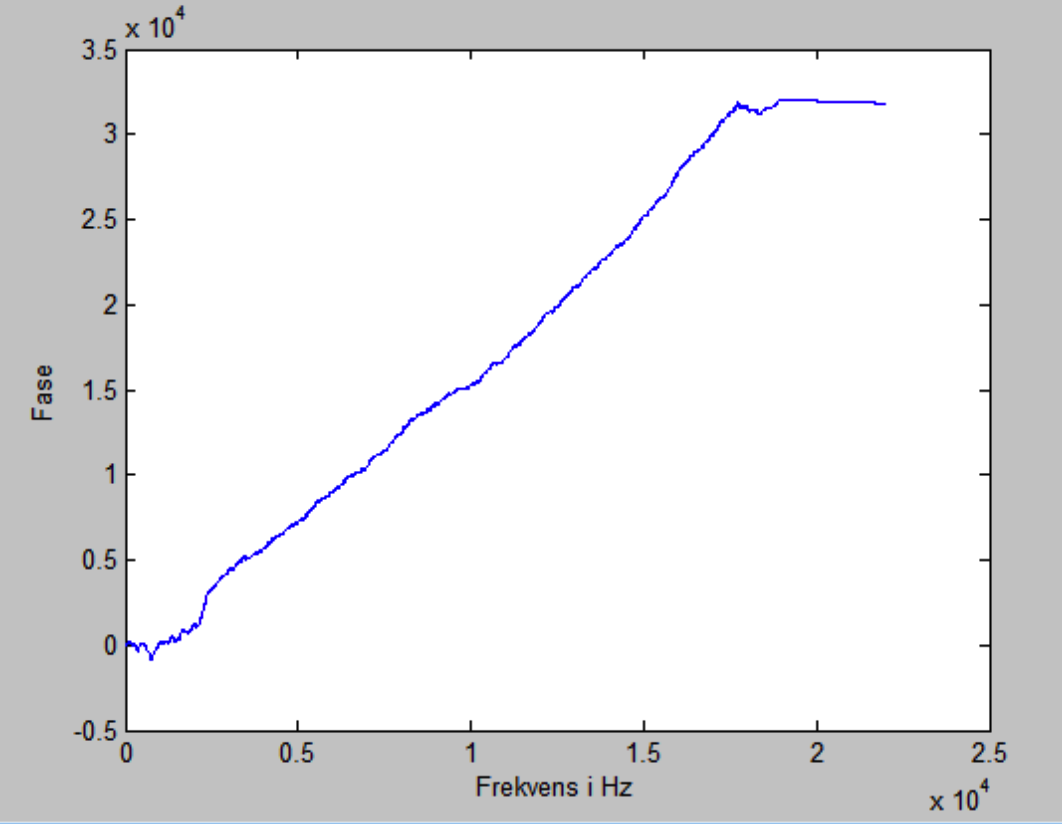
\includegraphics[width=0.8\textwidth]{Figur/Snip20151111_85}
	\caption{Fasen for det samlede signal, FFT}
\end{figure}

Hvis man tager det inverse af dette burde det bliver det samme, som det ufiltreret signal og det filtreret signal, hvor der ingen forstærkning var.
Dette plottes og sammenligningen kan ses på Figur 2.24, 2.25 og 2.26. 

\begin{figure}[H]
	\centering
	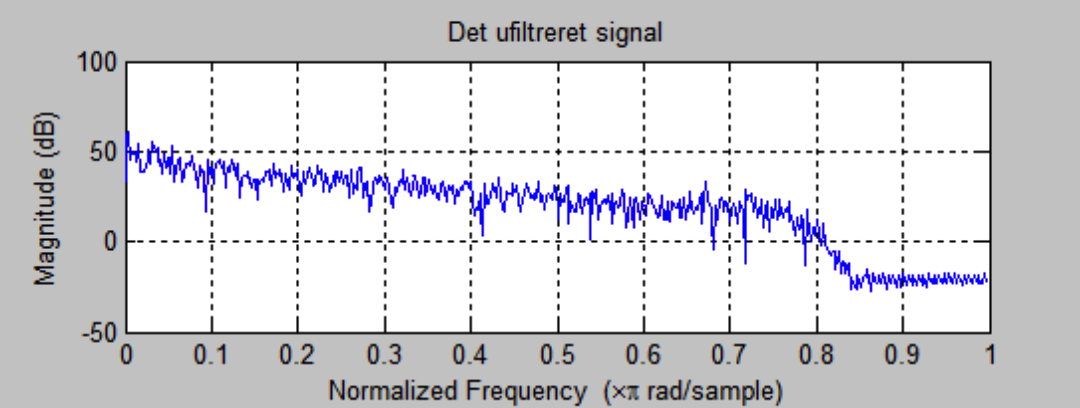
\includegraphics[width=0.8\textwidth]{Figur/Snip20151111_68}
	\caption{Det ufiltreret signal}
\end{figure}

\begin{figure}[H]
	\centering
	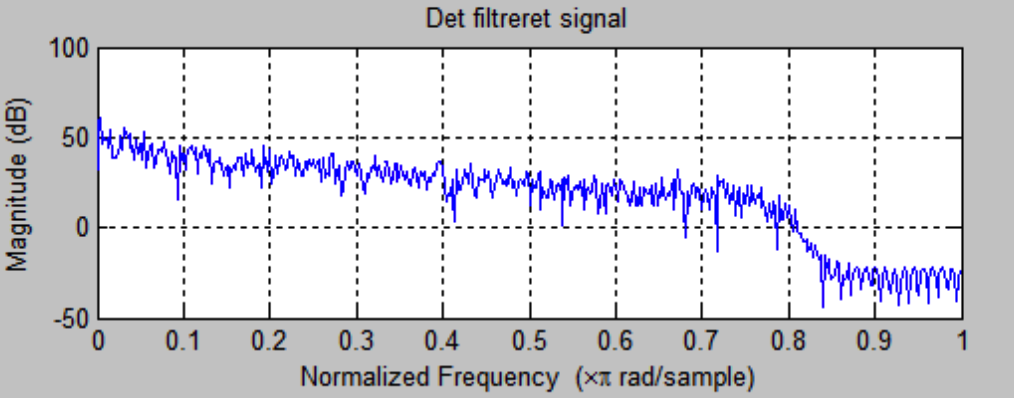
\includegraphics[width=0.8\textwidth]{Figur/Snip20151111_69}
	\caption{Det filtreret signal}
\end{figure}

\begin{figure}[H]
	\centering
	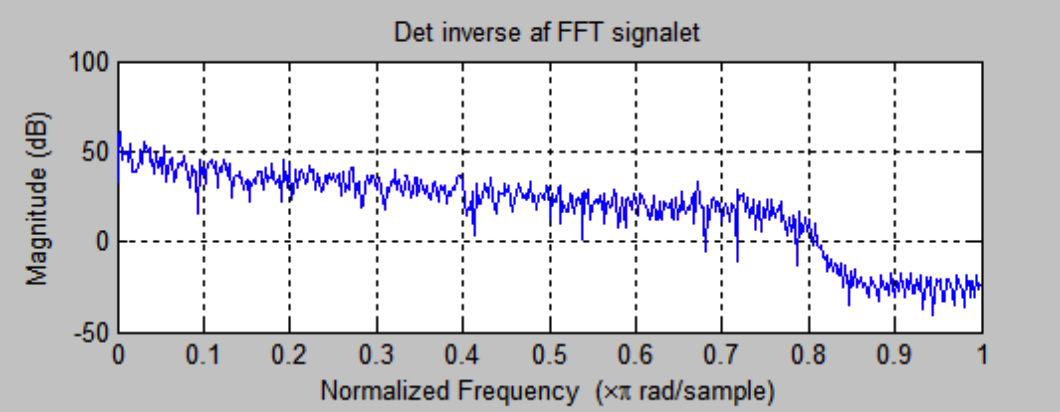
\includegraphics[width=0.8\textwidth]{Figur/Snip20151111_87}
	\caption{Det inverse af FFT signalet}
\end{figure}

Alle disse er ens, hvilket er det man forventede. 










